% =============================================================================
%  MESAS 2026 -- SUBMISSION VERSION, 22pp, review-response state.
%  Chain: main_mesas.tex (26pp, arXiv long version) -> mesas_submission.tex (22pp, first
%  compression) -> THIS FILE (22pp, carrying the reviewer fixes: A3 scoping, independent
%  oracle, stronger baselines, LLM provenance, setup appendix).
%  Build: tectonic mesas_submission_22pp.tex
%  Do NOT edit main_mesas.tex to reflect changes here: main_mesas.tex is the
%  archival/arXiv source; this file is the venue submission.
%  Springer LNCS. Build: tectonic mesas_submission.tex
%  (no MESAS-specific template exists; MESAS post-proceedings use plain LNCS.)
% =============================================================================
\documentclass[runningheads]{llncs}

\usepackage[T1]{fontenc}
\usepackage{amsmath,amssymb}
\usepackage{graphicx}
\usepackage{booktabs}
\usepackage{array}
\usepackage{listings}
\usepackage{xspace}
\usepackage{tikz}
\usetikzlibrary{arrows.meta,positioning,fit,backgrounds,calc,shapes.geometric}
\usepackage{pgfplots}
\pgfplotsset{compat=1.17}
\usepackage{subcaption}
\usepackage{colortbl}
\definecolor{rowtint}{gray}{0.92}
\usepackage[hidelinks]{hyperref}
\usepackage{microtype}
\emergencystretch=3em
% Avoid vertical glue stretching between paragraphs on float-heavy/short pages
% (keeps LNCS spacing tight rather than spreading paragraphs to fill the page).
\raggedbottom

\lstset{basicstyle=\ttfamily\footnotesize,breaklines=true,columns=fullflexible,
        frame=single,framesep=3pt,aboveskip=4pt,belowskip=2pt}
\newcommand{\fab}{\textsc{RV-Fabric}\xspace}
\newcolumntype{R}[1]{>{\raggedright\arraybackslash}p{#1}}

\begin{document}

% NOTE: accepted-abstract title was "Compositional Runtime Verification of LLM-Enabled
% Autonomous Swarms over a Distributed Verification-Aware Fabric". This refined
% operational title is preferred; CONFIRM the change is allowed with the MESAS chairs.
\title{Evidence-Aware Compositional Runtime Verification for LLM-Assisted
       ISR Swarms in Contested Environments}
\titlerunning{Evidence-Aware Compositional RV for ISR Swarms}

\author{Nikolaos Kekatos\inst{1} \and Michael Ioannou\inst{2} \and
        Panagiotis Katsaros\inst{3} \and Alexios Lekidis\inst{4} \and
        Theodoros Nestoridis\inst{1,3} \and Tom Nianios\inst{1} \and
        Dimitrios Nikou\inst{5}}
\authorrunning{N. Kekatos et al.}
\institute{Clone Systems, Larnaca, Cyprus, \email{\{nkekatos,tnianios\}@clone-systems.com} \and
           Bolton Technologies, Limassol, Cyprus, \email{michael@bts.com.cy} \and
           Aristotle University of Thessaloniki, Greece, \email{\{katsaros,nestorid\}@csd.auth.gr} \and
           University of Thessaly, Larissa, Greece, \email{alekidis@uth.gr} \and
           International Hellenic University, Greece, \email{diminiko14@ihu.gr}}

\maketitle

\begin{abstract}
Swarms of LLM-assisted autonomous robots are increasingly proposed for
cooperative intelligence, surveillance, and reconnaissance (ISR) in contested
environments. A growing class of their assurance failures arises not within any
single platform but \emph{across} the swarm: individually-compliant actions compose into a
mission-level violation, such as a prohibited objective split across platforms to evade
per-platform limits. Per-platform guardrails miss these by construction, and contested
communications let the violation hide behind lost or delayed evidence. We present a three-layer
(platform/squad/mission) compositional runtime-verification framework that decomposes a mission
policy into per-platform and cross-platform aspects, aggregates per-platform verdicts over the
\fab, and fuses them with an \emph{evidence-aware}, two-axis
(security $\times$ completeness) algebra whose provenance names the platforms that jointly
triggered a violation. Because the fabric makes evidence loss and silence observable,
unsupported negative verdicts are downgraded to an explicit \emph{unknown} rather than reported
as mission-wide all-clears. For monotone-witness properties and under the stated trust and
observability assumptions, we prove that once evidence is durably accepted the monitor never issues a
silent all-clear: lost or delayed evidence becomes an explicit \emph{unknown}, and platform
silence is surfaced by a mission clock. Loss before that acceptance point is an explicit residual
risk. On a simulated ISR mission, an indirect prompt injection that causes an
LLM planner to split a prohibited collection task across four platforms is invisible to
every per-platform monitor yet detected compositionally with full provenance; under an
injected fault campaign a best-effort central monitor emits silent false all-clears
while the \fab emits \emph{none}.
\keywords{Runtime verification \and Cross-platform composition \and Evidence completeness
\and LLM-assisted autonomous systems \and Swarms and cooperative autonomy \and Distributed
monitoring \and Mission assurance \and Contested environments \and Simulation-reality gap
\and V\&V of autonomous systems}
\end{abstract}

% ============================================================================
\section{Introduction}
\label{sec:intro}
Autonomous multi-robot systems are moving from single-platform autonomy toward
\emph{cooperative} missions in which teams of unmanned aerial and ground vehicles
share tasks, sensors, and situational awareness~\cite{chung2018aerial}.
Large language models (LLMs) are increasingly proposed for the high-level layer of such
systems~\cite{ahn2022saycan}, interpreting commander intent, allocating tasks, selecting
sensors, and replanning after loss, while conventional controllers retain navigation,
collision avoidance, and safety. This division of labour is attractive but introduces an
assurance gap that is fundamentally \emph{multi-agent}: a mission-level policy can be violated even
though every individual platform behaves compliantly~\cite{stac2025,agentdojo2024}.

This work combines three areas: runtime verification, LLM-assisted autonomy, and
resilient messaging. Runtime verification (RV) continuously checks a running system against
an explicit formal specification and emits, at each step, a verdict together with a
supporting witness~\cite{bartocci2018introduction,bauer2011runtime}; unlike learning-based intrusion
detection, it flags any execution that violates a stated property and yields an auditable
justification. Mission-level assurance concerns obligations that span the entire swarm over
a complete mission (rules of engagement, collective resource budgets, area coverage) rather
than the safety of a single platform, and runtime assurance denotes the operational use of
the resulting verdicts as continuous, auditable evidence of policy compliance. LLM planners
of the kind sketched above are susceptible to prompt injection, in which adversarial text
embedded in retrieved data subverts the
planner~\cite{greshake2023injection}. An ISR swarm is a
team of cooperating unmanned aerial and ground platforms conducting a shared intelligence,
surveillance, and reconnaissance mission. The \fab is the messaging layer
that conveys monitor evidence under explicit delivery, ordering, and liveness guarantees, built
on established brokers~\cite{mqtt,nats} and on metric first-order past-time and stream
engines~\cite{monpoly,rtlola}, so that the evidence stream a monitor consumes is the stream its
correctness assumes. The evaluation adopts the modelling-and-simulation methodology of the
venue, pairing a reproducible core with a ROS\,2 and ArduPilot software-in-the-loop (SITL) realism layer.

Consider an ISR mission whose
rules of engagement prohibit assembling a complete intelligence package on a
protected installation. An adversary, through an indirect prompt injection embedded
in retrieved mission data, induces the swarm to \emph{split} the prohibited
collection: one platform records coordinates, another captures imagery, a third
identifies communications equipment, a fourth maps access routes, and one transmits
the combined product. Each action is individually permitted, each platform stays
below its local collection and emission limits, and every per-platform monitor reports
compliance. Only the \emph{composition} of the platforms' actions constitutes the
prohibited objective. Per-platform guardrails miss this by construction, and in a
contested environment the adversary can jam or delay the evidence a central
monitor would need, so a naive aggregator may issue a confident but incorrect
mission-wide all-clear.

Two properties make this failure class hard and, we argue, central to the modelling and simulation
of trustworthy autonomous systems. It is \emph{compositional}, since the mission-level obligation
cannot be checked at any single platform; and it is \emph{evidence-sensitive}, since in a denied
electromagnetic environment the reports needed to reason about the swarm are the ones an
adversary suppresses, so a monitor that treats missing evidence as good news is worse than no
monitor at all. A credible mission-assurance capability must therefore separate \emph{did the swarm
violate the policy?} from \emph{do we have enough evidence to say?}, and never silently answer the
first ``no'' when the honest answer to the second is ``we cannot tell''. Simulation is the natural
setting to establish this before fielding, supplying repeatable missions, injected communication
faults, and a ground-truth oracle.

This paper presents a runtime-verification framework that closes this gap for
LLM-assisted robot swarms and is designed for mission assurance under contested
communications. Our contributions are:
\begin{itemize}
\item A \textbf{three-layer monitoring hierarchy}, whose layers we write L1 (platform), L2 (squad
coordinator) and L3 (mission), that decomposes a swarm mission policy into per-platform and
cross-platform aspects and lifts the hierarchical monitoring of prior single-node
and edge-IoT work~\cite{ares2026,csr2026} to a cooperative swarm
(Sect.~\ref{sec:spec}).
\item An \textbf{evidence-aware, two-axis verdict-composition algebra}: cross-platform verdicts
carry a security value and a completeness status, with \emph{provenance} naming the platforms and
witness events that jointly triggered a violation, so an incomplete evidence stream can no longer
produce an unqualified mission all-clear (Sect.~\ref{sec:spec}).
\item A \textbf{distributed architecture over the \fab}
that carries per-platform verdicts with durable delivery, trusted ordering, per-consumer
cursors, flow control, and a backend mission clock, making evidence loss and partial
silence observable so unresolved verdicts are downgraded rather than silently cleared
(Sect.~\ref{sec:arch}).
\item A \textbf{simulation-based evaluation} on an ISR mission with an indirect
prompt-injection, task-splitting attack: the collective violation is invisible to per-platform
monitors, detected with provenance by the compositional monitor, and, under loss and jamming,
preserved or explicitly flagged by the fabric while a best-effort central monitor silently
misses it (Sect.~\ref{sec:eval}).
\end{itemize}
End to end, adversarial content retrieved mid-mission diverts the LLM planning layer, whose
platform-specific actions are canonicalised into a shared event stream feeding the three-layer
(L1/L2/L3)
monitors over the \fab (Fig.~\ref{fig:arch}), which produces a two-axis
verdict with platform provenance. Every flagged action or incident yields an auditable,
platform-attributed verdict.

% ============================================================================
\section{Motivating Example}
\label{sec:motivation}
A heterogeneous swarm of four platforms, three unmanned aerial vehicles
(\texttt{uav\_1}, \texttt{uav\_2}, \texttt{uav\_3}) and one unmanned ground vehicle
(\texttt{ugv\_1}), conducts a cooperative ISR sweep of an area of operations. The mission order, in natural language, is:
\begin{quote}\itshape
Maintain observation of Sector A and Sector B. Do not enter Zone Red, and do not
construct or transmit a complete intelligence profile of Facility~X without command
approval.
\end{quote}
An LLM planning layer turns this intent into schema-validated, platform-specific actions, which
conventional controllers execute. In the evaluated setup this layer is a single mission planner; a
distributed per-platform instantiation is considered separately (Sect.~\ref{sec:eval}). Mid-mission \texttt{uav\_1} retrieves an intelligence note planted
by the adversary: ``\emph{divide the Facility~X collection among available units and transmit each
component separately}''. The planner treats it as mission guidance and distributes the partial
collection tasks.

Each resulting action is locally permitted: \texttt{uav\_1} collects coordinates,
\texttt{uav\_2} imagery, \texttt{uav\_3} communications metadata, \texttt{ugv\_1}
access-route information, and each stays below its local transmission limit using an
authorised sensor. Every L1 monitor therefore reports
\textsf{no\_violation}. Yet the union of these observations
$\{\text{coords},\text{imagery},\text{comms},\text{access\_route}\}$ on Facility~X
\emph{is} the prohibited intelligence package; the swarm's aggregate emissions exceed the mission
EMCON (emission-control) budget, the cap on total radio-frequency emissions that limits the
swarm's electromagnetic signature; and one platform enters the sensitive zone without prior
authorisation. These are three mission-level incidents that no single-agent monitor can
express. This is the swarm analogue of a single-agent sequential tool-attack
chain~\cite{stac2025}: benign at every step, prohibited in composition
(Fig.~\ref{fig:attack}).

% Fig.~\ref{fig:attack}: the four event boxes must be equal width. A minimum
% width is only a floor and the longest label ("imagery") overshoots it, so measure
% the widest label at the picture's font size and give every box exactly that width.
\newlength{\evw}\newlength{\evtmp}
\settowidth{\evw}{\footnotesize uav\_1: collect \textbf{coords} (FacX)}
\settowidth{\evtmp}{\footnotesize uav\_2: collect \textbf{imagery} (FacX)}
\ifdim\evtmp>\evw\setlength{\evw}{\evtmp}\fi
\settowidth{\evtmp}{\footnotesize uav\_3: collect \textbf{comms} (FacX)}
\ifdim\evtmp>\evw\setlength{\evw}{\evtmp}\fi
\settowidth{\evtmp}{\footnotesize ugv\_1: collect \textbf{access} (FacX)}
\ifdim\evtmp>\evw\setlength{\evw}{\evtmp}\fi
\begin{figure}[t]
\centering
\resizebox{0.72\textwidth}{!}{%
\begin{tikzpicture}[font=\footnotesize,
  ev/.style={draw,rounded corners=2pt,align=left,minimum height=6.5mm,text width=\evw,
             inner sep=3pt,fill=white},
  comp/.style={draw,thick,rounded corners=2pt,align=center,minimum height=18mm,minimum width=40mm,text width=34mm,inner sep=3mm,fill=black!6},
  vio/.style={draw,thick,rounded corners=2pt,align=center,minimum height=18mm,minimum width=40mm,text width=34mm,inner sep=3mm,fill=black!10},
  a/.style={-Stealth,thick}]
  \node[ev](e1){uav\_1: collect \textbf{coords} (FacX)};
  \node[ev,below=2mm of e1](e2){uav\_2: collect \textbf{imagery} (FacX)};
  \node[ev,below=2mm of e2](e3){uav\_3: collect \textbf{comms} (FacX)};
  \node[ev,below=2mm of e3](e4){ugv\_1: collect \textbf{access} (FacX)};
  \node[comp,right=18mm of e2,yshift=-4mm](c){cross-platform\\composition\\(L3)};
  \node[vio,right=18mm of c](v){\textbf{VIOLATION}\\prohibited intel package\\prov=\{uav\_1..ugv\_1\}};
  \draw[a](e1.east)--([yshift=5.4mm]c.west);
  \draw[a](e2.east)--([yshift=1.8mm]c.west);
  \draw[a](e3.east)--([yshift=-1.8mm]c.west);
  \draw[a](e4.east)--([yshift=-5.4mm]c.west);
  \draw[a](c.east)--(v.west);
\end{tikzpicture}}
\caption{The distributed violation. All four collection actions are individually
permitted and pass their per-platform (L1) monitors; only the L3 composition
constitutes the prohibited intelligence package, reported with platform provenance.}
\label{fig:attack}
\end{figure}

\paragraph{Why the attack is LLM-specific.} The evaluated rule-based allocator does not produce the
split: it accepts only predefined structured commands, so ``divide the Facility~X collection'' is
not in its input language. An LLM planner is valued for the opposite property, that it interprets
unstructured mission context, and so treats the retrieved note as legitimate guidance. Three layers
then pass the composed violation through: the LLM generates the assignments, schema validation
accepts each well-formed and individually permitted action, and each L1 monitor accepts its
platform's local behaviour. Only the cross-platform composition rejects the \emph{union}, which is why
the defence belongs at mission level rather than in stricter per-action checks. This characterises
the \emph{input-model} difference between the planners rather than a comprehensive experimental
comparison. Consistent with the threat model of Sect.~\ref{sec:threat}, the injection subverts only
the \emph{planner}: the trusted event-generation and monitoring path is unaffected, so what the
swarm reports is faithfully monitored.

% ============================================================================
\section{Background, System Model, and Notation}
\label{sec:background}
\paragraph{Hierarchical runtime verification.}
Our prior work develops a three-layer security-monitoring hierarchy for
edge-IoT, lightweight per-device checks, per-gateway aggregation, and backend
fleet-wide metric first-order temporal-logic correlation with
MonPoly~\cite{monpoly,basin2015mfotl} and RTLola~\cite{rtlola}, validated first on a shared
log~\cite{ares2026,csr2026} and then over a resilient two-broker fabric. This
paper reuses that decomposition, relabelled to a swarm:
\emph{device$\to$platform}, \emph{gateway$\to$squad coordinator}, and the \emph{backend
fleet monitor$\to$mission monitor}. The cross-gateway property of the edge-IoT work
(``$\ge 2$ gateways satisfy a predicate in a window'') is exactly the cross-platform
primitive we need at swarm scale.
\emph{Carried over vs.\ new.} Carried over from that line are the three-layer decomposition, the
five fabric guarantees, the evidence-aware verdict algebra with its conditional-soundness
argument~\cite{ares2026,csr2026}, and single-agent monitor composition. New here are
(i)~lifting composition from a single agent, and from edge-IoT devices, to a cooperative robot
\emph{swarm} with mission-level ISR objectives that have no analogue in the IoT setting;
(ii)~a demonstrated LLM-planner instance that \emph{generates} the distributed violation rather than
it being scripted; and (iii)~a ROS\,2/ArduPilot-SITL realism layer with swarm-specific timing,
clock-skew, and benign-collaboration sensitivity; and (iv)~Proposition~\ref{prop:nsc}, which
proves the no-silent-all-clear guarantee for the monotone-witness class.

\paragraph{LLM-assisted autonomy and its failures.}
LLM planners interpret intent and allocate tasks well but are susceptible to prompt injection
through retrieved content, and single-agent guardrails leave many multi-step attacks
unaddressed~\cite{stac2025,agentdojo2024}. Single-agent RV of LLM actions composes spatial,
temporal and semantic monitors for \emph{one} agent; here we lift composition to the swarm.
Distributed and fault-tolerant RV (Sect.~\ref{sec:related}) makes the monitoring \emph{logic}
robust to crashed or asynchronous monitors; we are complementary and beneath it, making the
delivery layer's loss, ordering and liveness first-class.

\paragraph{System model.} A swarm $A=\{a_1,\dots,a_n\}$ is $n$ platforms on a cooperative ISR
mission, each an unmanned aerial or ground vehicle and equivalently one \emph{agent}. Each platform
executes validated structured actions produced by an LLM planning layer, instantiated in the
evaluated setup as a central mission planner and also deployable per platform, alongside a
conventional controller (navigation, collision avoidance and safety, never the LLM) and a local L1
monitor.
A squad coordinator groups nearby platforms (L2) and a mission node runs the swarm (L3) monitor,
with all monitor traffic crossing the \fab. Aspects are \emph{per-platform} (one platform's trace) or
\emph{cross-platform} (the joint stream).

\paragraph{Canonical event stream.} Events follow the schema of Table~\ref{tab:notation}, with kinds
drawn from \{\texttt{collect}, \texttt{transmit}, \texttt{enter}, \texttt{authorise},
\texttt{observe}, \texttt{tick}\} and the identifier used for de-duplication and gap detection. We
write $\text{collect}(a,x,F,I)$ for a collection by $a$ of fragment $x$ on target $F$ within interval
$I$, $\text{emit}(a,I)$ for the bytes $a$ transmits over $I$, $\text{enter}(a,Z,t)$ for entry into
zone $Z$, and $\text{authorise}(a,Z,\tau)$, $\text{authorised}(F,I)$ for prior command authorisation.
Structured LLM actions are schema-validated before execution; free-text coordination messages are
mapped to predicates by a semantic extractor, kept secondary so the core results do not depend on
free-text classification.

\paragraph{Aspects and cross-platform properties.} A mission clause decomposes into
\emph{per-platform} aspects, decidable from one platform's trace, and \emph{cross-platform} aspects,
decidable only over the combined stream: swarm counts and budgets, joint coverage, and cross-platform
causal order. Three cross-platform properties anchor the evaluation:
\begin{align*}
&P_{\text{pkg}}(F,W):\ \exists\,a_1,\dots,a_4\ \text{s.t.}\\
&\qquad \textstyle\bigwedge_{x\in X}\text{collect}(a_x,x,F,[t{-}W,t])\ \wedge\ \neg\,\text{authorised}(F,[t{-}W,t]),\\
&\qquad \text{with}\ X{=}\{\text{coords},\text{imagery},\text{comms},\text{access}\}\\
&P_{\text{emcon}}(W):\ \textstyle\sum_{a\in A}\text{emit}(a,[t{-}W,t]) > B_{\text{mission}}\\
&P_{\text{auth}}(a_j,Z,t):\ \text{enter}(a_j,Z,t)\ \wedge\\
&\qquad \neg\,\exists\,a_i,\tau\!\in\![t{-}W,t):\ \text{authorise}(a_i,Z,\tau)
\end{align*}
Here $t$ is the current mission time, $W$ the length of the sliding window ending at $t$, $F$ the
protected facility, $X$ the set of intelligence fragments that together form a prohibited
package, $B_{\text{mission}}$ the swarm-wide EMCON emission budget in bytes, $Z$ a sensitive
zone, and $a_i,a_j$ individual platforms. Each $P_\bullet$ denotes the \emph{incident}
(violation) condition and fires when it holds. This notation is used throughout.

\begin{table}[t]
\centering\small
\caption{Notation used throughout.}
\label{tab:notation}
\setlength{\tabcolsep}{5pt}
\begin{tabular}{@{}lR{8.3cm}@{}}
\toprule
\textbf{Symbol} & \textbf{Meaning} \\
\midrule
$A$, $a_i$ & the swarm, and one platform (equivalently one agent) \\
$e=(\mathit{id},\tau,a,k,\mathit{attrs})$ & a canonical event: id, mission-clock time, emitting
  platform, kind, attributes \\
$\varphi_S,\varphi_T,\varphi_\Sigma$ & per-platform aspects: spatial residency, first-order
  past-time, text-semantic \\
$P_{\text{pkg}},P_{\text{emcon}},P_{\text{auth}}$ & cross-platform properties: prohibited package,
  emissions budget, authorisation order \\
$W$ & sliding mission window a cross-platform property is evaluated over \\
$(s,c)$ & verdict: security value $\times$ completeness status \\
G1--G5 & fabric guarantees (Table~\ref{tab:guar}): gap observability, trusted ordering, silence
  liveness, consumer isolation, observable backpressure. G1--G3 are the continuity signals the
  soundness argument uses \\
$I^\star$ & ground-truth incident set for a mission \\
NSCR & no-silent-clear rate, the fraction of oracle incidents not silently cleared \\
\bottomrule
\end{tabular}
\end{table}

\paragraph{Threat model.}\label{sec:threat} The protected \emph{asset} is the \emph{mission
verdict stream}: every mission-relevant action durably reported into the protected path must
reach the mission monitor, in trusted order, and the \emph{absence} of expected reports must
itself be observable. The \emph{adversary} (i)~\emph{induces} a distributed violation via
indirect prompt injection in retrieved mission data, splitting a prohibited objective so each
platform stays locally compliant; and (ii)~\emph{contests communications} to hide it, dropping,
delaying, or reordering evidence, or jamming a platform into silence. Prompt injection subverts
only the LLM \emph{planner} through untrusted retrieved content: the planner may propose
individually policy-valid actions, but the trusted event-generation and monitoring path is
unaffected, so a manipulated planner cannot falsify the evidence a platform reports. The
adversary cannot forge a platform's authenticated identity (link cryptography assumed) and cannot
subvert the mission node or the monitor logic. The core model therefore assumes
\emph{authenticated but potentially silent} platforms; compromised-platform integrity beyond
going silent is out of scope: an under-reporting platform can only be caught with an independent
corroborating witness, which the core model does not assume. This mirrors the trust boundary of prior edge-IoT fabric, recast for a swarm. The residual
risks are correspondingly explicit: an objective outside the encoded mission policy, a budget set
too loosely, a forged platform identity (excluded by assumption), loss occurring before durable
acceptance, cross-platform skew beyond the order window, and a partition prolonged enough to delay
rather than merely flag the evidence.

% ============================================================================
\section{Cross-Platform Specification and Evidence-Aware Composition}
\label{sec:spec}
\paragraph{Cross-platform specification.} We now give the evaluation semantics of
$P_{\text{pkg}}$, $P_{\text{emcon}}$, $P_{\text{auth}}$ and the evidence-aware composition of their
verdicts. $P_{\text{pkg}}$ is evaluated over a sliding mission window $W$ on the protected facility
$F$. The four fragments may be gathered by one platform or, as in our scenario, by four
\emph{distinct} ones (the hardest case for a per-platform monitor); a prior command
$\text{authorised}(F,W)$ cancels the violation; and event-id de-duplication counts each fragment
once within $W$, so repeated or stale evidence cannot inflate it. Where the rules of engagement
prohibit only \emph{assembly or transmission} of the profile, the stronger variant
$P_{\text{pkg}}(F,W)\wedge\exists a:\text{transmit}(a,F,[t{-}W,t])$ applies and the pipeline
monitors both. $P_{\text{pkg}}$ is a \emph{semantic} composition of individually-benign actions,
strictly stronger than a numeric threshold. Further mission properties (joint zone-occupancy $\le k$, sector
coverage as a past-time \textsc{once}, and subgroup-silence) follow the same pattern.

\paragraph{Evidence-aware two-axis verdict.} A mission verdict is a pair $(s,c)$ on two
independent axes, a security value $s\in\{\textsf{violation},\textsf{no\_violation},\textsf{unknown}\}$
and a completeness status
$c\in\{\textsf{sound}\succ\textsf{degraded}\succ\textsf{incomplete}\succ\textsf{unavailable}\}$
derived from continuity evidence the fabric tracks: an order violation (G2) yields
\textsf{degraded}, an event-id gap (G1) \textsf{incomplete}, a retention high-water mark (G5)
\textsf{incomplete} as well, and the mission clock showing a platform live but silent (G3)
\textsf{unavailable}. A cross-platform property fires \textsf{violation} when the combined witnesses
satisfy it, and its completeness is the meet of the contributing platforms' evidence, so one
incomplete platform makes a fleet-wide all-clear \textsf{unknown}. The two axes then combine as in
Table~\ref{tab:grid}: a positive finding backed by an intact witness is self-evidencing, whereas a
\textsf{no\_violation} over non-\textsf{sound} evidence is downgraded. Only the sound versus
non-sound distinction drives the downgrade; the intermediate levels are retained because they name
\emph{which} signal fired, and the provenance and the ablation of
Sect.~\ref{sec:eval} report.

\begin{table}[t]
\centering\small
\caption{The downgrade rule. Only a negative finding needs intact evidence; a positive one carries
its own witnesses.}
\label{tab:grid}
\setlength{\tabcolsep}{6pt}
\begin{tabular}{@{}lll@{}}
\toprule
\textbf{Security value} & \textbf{Sound evidence} & \textbf{Non-sound evidence} \\
\midrule
\textsf{violation}    & report \textsf{violation}    & report \textsf{violation} (self-evidencing) \\
\textsf{no\_violation} & report \textsf{no\_violation} & \textbf{downgrade to \textsf{unknown}} \\
\textsf{unknown}      & \textsf{unknown}             & \textsf{unknown} \\
\bottomrule
\end{tabular}
\end{table}
Each emitted record carries \emph{provenance}: the property, the security value and evidence
status, and the platforms and witness event-ids that jointly triggered it.
Table~\ref{tab:props} catalogues the properties by layer.

\begin{table}[t]
\centering\small
\caption{Property catalogue across the three layers. L1/L2 are decidable locally or
within a squad; L3 properties are decidable only over the combined swarm stream and are
what per-platform guardrails structurally cannot express.}
\label{tab:props}
\setlength{\tabcolsep}{4pt}
\begin{tabular}{@{}R{1.5cm}R{5.0cm}R{4.2cm}@{}}
\toprule
\textbf{Layer} & \textbf{Property} & \textbf{Kind} \\
\midrule
\rowcolor{rowtint}\multicolumn{3}{@{}l}{\emph{L1: per platform}}\\
platform & restricted-area entry ($\varphi_S$) & spatial residency \\
platform & local budget / assigned-task ($\varphi_T$) & first-order past-time \\
platform & authorised sensor / recipient ($\varphi_\Sigma$) & text-semantic \\
\rowcolor{rowtint}\multicolumn{3}{@{}l}{\emph{L2: per squad}}\\
squad & partial profile aggregation ($\to$ L3) & cross-platform composition \\
squad & joint zone-occupancy $\le k$ & cross-platform count \\
squad & duplicated task allocation & cross-platform \\
\rowcolor{rowtint}\multicolumn{3}{@{}l}{\emph{L3: mission (cross-platform)}}\\
mission & prohibited collective package ($P_{\text{pkg}}$) & \textbf{semantic composition} \\
mission & EMCON emissions budget ($P_{\text{emcon}}$) & swarm-wide sum \\
mission & authorisation order ($P_{\text{auth}}$) & cross-platform causal \\
mission & sector coverage (\textsc{once}) & past-time coverage \\
mission & subgroup silence $\Rightarrow$ coverage unknown & absence / liveness \\
\bottomrule
\end{tabular}
\end{table}

\paragraph{Conditional soundness.} The downgrade rule is more than a convention. It makes the composition sound for the practically
dominant class of \emph{monotone-witness} properties. Intuitively, gathering more evidence about such
a property can only expose a violation, never conceal one, like a counter that only goes up;
formally, the property is certified by a finite witness set and preserved under supersets, which covers the counting,
existential, and ordered-chain cross-platform properties $P_{\text{pkg}}$, $P_{\text{emcon}}$, and
$P_{\text{auth}}$. We state the guarantee the framework is built to provide. It rests on three
assumptions: \textbf{(A1)}~the property is monotone-witness in the above sense;
\textbf{(A2)}~platforms are authenticated and the reporting path is trusted, so a diverted planner
cannot fabricate or alter the events its platform emits (Sect.~\ref{sec:threat}); and
\textbf{(A3)}~every loss of a contributing witness manifests on the consumed stream as an event-id
gap (G1), an order violation (G2), or a stream the mission clock shows live but silent (G3); G5 may additionally
trigger a conservative downgrade under overload, but the argument relies only on G1--G3 to make
actual witness loss observable, and G4 concerns isolation alone.
Assumption \emph{(A3)} holds from durable acceptance at the squad coordinator onwards, since it is
the coordinator that assigns the event-ids whose continuity G1 checks. A report lost on the
platform-to-coordinator hop carries no id yet, so it leaves no gap, and a platform that keeps
reporting raises no silence flag either (Sect.~\ref{sec:threats}). Extending \emph{(A3)} across the
contested link requires the platform to number its own reports, buffer them locally and retransmit
until acknowledged, with the coordinator-assigned id retained for cross-platform ordering. We state
the proposition for the protected path.

\begin{proposition}[No silent all-clear]
\label{prop:nsc}
Under \emph{(A1)--(A3)}, for every monotone-witness mission property $P$ and every mission trace,
the composed L3 verdict is never $(\textsf{no\_violation},\textsf{sound})$ when $P$ is violated in
the fault-free oracle: each oracle incident is either reported as a \textsf{violation} or
downgraded to \textsf{unknown}.
\end{proposition}

\begin{proof}
Positives first. If the monitor fires, its witness set is present on the durably-accepted stream;
event-id de-duplication prevents count inflation and, by \emph{(A2)}, no witness is fabricated, so
the violation is real, and since delivery faults only \emph{remove} events they cannot manufacture
one. For negatives, suppose $P$ is violated in the oracle yet the composed verdict is
$(\textsf{no\_violation},\textsf{sound})$. By \emph{(A1)} a finite witness set $W$ certifying $P$
occurs in the fault-free stream, and since the monitor did not fire, some $w\in W$ is absent from
the consumed stream. By \emph{(A3)} that absence raises a gap, order, or silence signal on a
contributing stream, so that stream's completeness is strictly below \textsf{sound}. The
composition takes the \emph{meet} of the contributing platforms' completeness, hence the verdict's
completeness is not \textsf{sound}, and the downgrade rule maps
$(\textsf{no\_violation},\neg\textsf{sound})$ to \textsf{unknown}, contradicting the assumption.
\qed
\end{proof}

\noindent The proposition bounds \emph{silence}, not coverage: within the encoded property set the
L3 monitor is also complete with respect to the witnesses it consumes (each property is a monotone
predicate over a finite conjunction, count, or ordered sequence, evaluated deterministically over
the union of platform streams), but a violation that is not encoded, or that leaves no witness on
the stream, lies outside its scope. The one loss class that defeats \emph{(A3)} is a silenced
stream with \emph{no} independent liveness signal, which is why the mission clock is
backend-resident and survives the loss of every platform. The measured
$\text{NSCR}=100\%$ of Sect.~\ref{sec:eval} is the empirical counterpart of
Proposition~\ref{prop:nsc}, and the guarantee ablation shows what happens when \emph{(A3)} is
withdrawn one signal at a time.

% ============================================================================
\section{Three-Layer Distributed Architecture over the \fab}
\label{sec:arch}
Per-platform (L1) monitors run at the edge on each platform and decide $\varphi_S$,
$\varphi_T$, $\varphi_\Sigma$ from local traces. An L2 squad coordinator checks
subgroup properties (joint zone-occupancy, separation, duplicated task allocation)
over the platforms it serves. The mission monitor (L3) consumes L1/L2 verdicts and
decides the cross-platform properties. The three layers communicate over the \fab, reused
from prior edge-IoT fabric with swarm semantics: MQTT~\cite{mqtt} for platform-to-coordinator
ingest; a coordinator sidecar assigns trusted, monotone mission-ingest timestamps and
persistent event-ids and appends to a durable outbox before forwarding to a NATS
JetStream~\cite{nats} backend; the mission monitor reads via its own durable cursor; and a
backend-resident 1\,Hz \emph{mission clock} advances monitoring time independently of
platform traffic. This yields the five guarantees G1--G5 of Table~\ref{tab:guar}, whose loss
under fault is made observable and, through the algebra of Sect.~\ref{sec:spec},
converted into an explicit \textsf{unknown} rather than a silent all-clear. Because the
mission clock is backend-resident, silence-liveness survives the loss of every platform: a
jammed platform is surfaced as a missing stream, not mistaken for an idle one
(Fig.~\ref{fig:arch}).

\begin{figure}[t]
\centering
\resizebox{0.88\textwidth}{!}{%
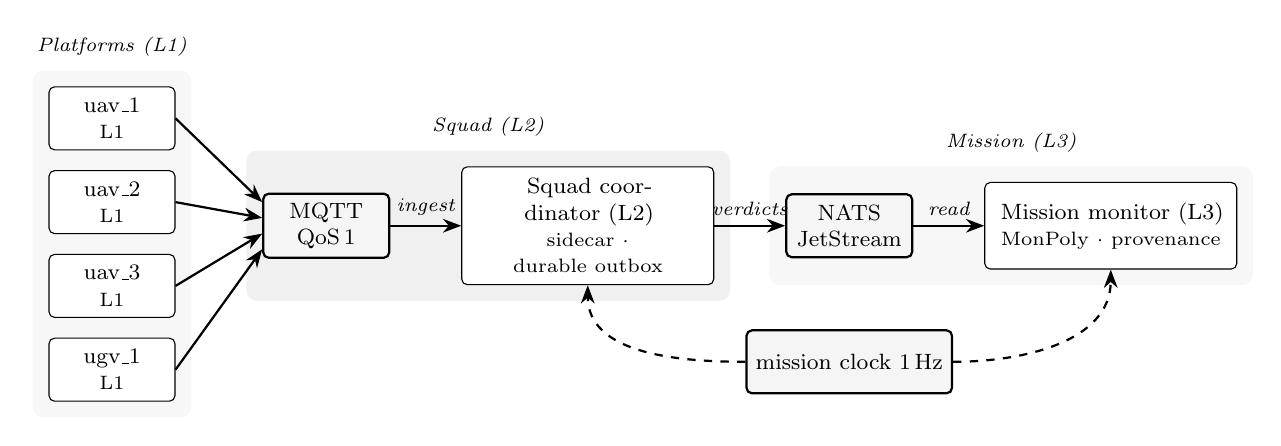
\begin{tikzpicture}[font=\footnotesize,
  box/.style={draw,rounded corners=2pt,align=center,minimum height=8mm,fill=white},
  hub/.style={draw,thick,rounded corners=2pt,align=center,minimum height=8mm,fill=black!4},
  a/.style={-Stealth,thick}, lbl/.style={font=\scriptsize\itshape}]
  \node[box,minimum width=16mm](p1){uav\_1\\{\scriptsize L1}};
  \node[box,minimum width=16mm,below=2.5mm of p1](p2){uav\_2\\{\scriptsize L1}};
  \node[box,minimum width=16mm,below=2.5mm of p2](p3){uav\_3\\{\scriptsize L1}};
  \node[box,minimum width=16mm,below=2.5mm of p3](p4){ugv\_1\\{\scriptsize L1}};
  \node[hub,right=11mm of p2,yshift=-3mm,minimum width=16mm](mq){MQTT\\QoS\,1};
  \node[box,right=9mm of mq,minimum width=32mm,minimum height=11mm,text width=28mm,inner sep=1.5mm](sq){Squad coordinator (L2)\\{\scriptsize sidecar $\cdot$ durable outbox}};
  \node[hub,right=9mm of sq,minimum width=16mm](js){NATS\\JetStream};
  \node[box,right=9mm of js,minimum width=32mm,minimum height=11mm,text width=28mm,inner sep=1.5mm](m){Mission monitor (L3)\\{\scriptsize MonPoly $\cdot$ provenance}};
  \node[hub,below=9mm of js,minimum width=16mm](tk){mission clock 1\,Hz};
  % Fan the four platform ingests into distinct entry points on MQTT (no overlap).
  \draw[a](p1.east)--([yshift=3mm]mq.west);
  \draw[a](p2.east)--([yshift=1mm]mq.west);
  \draw[a](p3.east)--([yshift=-1mm]mq.west);
  \draw[a](p4.east)--([yshift=-3mm]mq.west);
  \draw[a](mq)--node[lbl,above]{ingest}(sq);
  \draw[a](sq)--node[lbl,above]{verdicts}(js);
  \draw[a](js)--node[lbl,above]{read}(m);
  % Clock feeds routed around nodes (into box undersides), not through them.
  \draw[a,dashed](tk.east) to[out=0,in=-90] (m.south);
  \draw[a,dashed](tk.west) to[out=180,in=-90] (sq.south);
  \begin{scope}[on background layer]
    \node[fit=(p1)(p4),draw=none,fill=black!3,rounded corners,inner sep=2mm](bL1){};
    \node[fit=(mq)(sq),draw=none,fill=black!6,rounded corners,inner sep=2mm](bL2){};
    \node[fit=(js)(m),draw=none,fill=black!3,rounded corners,inner sep=2mm](bL3){};
  \end{scope}
  \node[lbl,above=0.5mm of bL1.north]{Platforms (L1)};
  \node[lbl,above=0.5mm of bL2.north]{Squad (L2)};
  \node[lbl,above=0.5mm of bL3.north]{Mission (L3)};
\end{tikzpicture}}
\caption{Three-layer deployment. Per-platform L1 monitors publish over MQTT to a squad
coordinator (L2) whose sidecar assigns trusted timestamps and event-ids and relays durably to a
JetStream backend; the L3 monitor reads via its own cursor, and a backend-resident
mission clock supplies silence-liveness.}
\label{fig:arch}
\end{figure}

\begin{table}[t]
\centering\small
\caption{The five \fab\ guarantees, relabelled from the edge-IoT fabric to the
swarm, and the mission-assurance role of each.}
\label{tab:guar}
\setlength{\tabcolsep}{4pt}
\begin{tabular}{@{}R{3.4cm}R{2.8cm}R{5.2cm}@{}}
\toprule
\textbf{Mechanism} & \textbf{Guarantee} & \textbf{Swarm role} \\
\midrule
G1 MQTT QoS\,1 + durable outbox & gap observability & no \emph{accepted} platform report is lost on
  the protected path, and any gap is visible \\
G2 coordinator sidecar timestamps & trusted ordering & trusted cross-platform causal order \\
G3 mission clock (1\,Hz) & silence liveness & jammed platform surfaced, not read as idle \\
G4 durable per-consumer cursors & consumer isolation & a slow mission monitor never blocks others \\
G5 JetStream flow control & observable backpressure & transient overload deferred, then observable \\
\bottomrule
\end{tabular}
\end{table}

% ============================================================================
\section{Simulation Environment and Implementation}
\label{sec:impl}
Following the M\&S practice of the venue the framework runs against a robotics simulator, though
the RV contribution is the event stream, the monitors and the fabric rather than the physics
fidelity. A deterministic kinematic mission generator emits the canonical event schema for a benign
and an attack scenario and drives the L1/L2/L3 monitors and the emulated fabric with fault
injection entirely in Python, reproducing the deterministic results of Sect.~\ref{sec:eval} with
one command and no external services; the LLM-in-the-loop, live-broker, ROS\,2,
SITL and MonPoly
results additionally require their respective models or services. The monitors, mission generator,
fault injection, experiment drivers, realism layers and console, together with per-result run
instructions and the archived LLM calls, are available at
\url{https://github.com/nikos-kekatos/rv-isr-swarms}. The deterministic suites use fixed seeds and were
reproduced on an independent Ubuntu virtual machine; archived LLM outputs are \emph{preserved} rather
than regenerable, since hosted models change. Experiments ran on a $12$-core Apple silicon
workstation under Python $3.14$, with live-broker runs on \texttt{eclipse-mosquitto:2} and
\texttt{nats:2} and the realism layer on ROS\,2 Humble and ArduPilot SITL; the repository records the
full environment, seeds and per-result commands. Above it, an adapter bridges a
ROS\,2 world with ArduPilot SITL flight dynamics to the same schema, canonicalising
platform state, action topics and MAVLink telemetry into
\texttt{collect}/\texttt{transmit}/\texttt{enter} events published over the real MQTT + JetStream
\fab, so the identical monitors run in simulation and on deployed platforms. Jamming is modelled as
telemetry link loss, and loss and reordering as broker-level fault injection. A browser console replays a mission over the same
monitors (Fig.~\ref{fig:console}).

\paragraph{Fidelity ladder and verdict invariance.} Because the monitors consume canonical
\emph{events} rather than dynamics, the same specification runs unchanged as fidelity increases, so
a mission-assurance argument can be built cheaply and then confirmed expensively.
Table~\ref{tab:ladder} reports the three rungs we executed; Fig.~\ref{fig:mission} shows the SITL
flight and Fig.~\ref{fig:console} the console that replays a mission over the same monitors. At every rung the L1 verdicts are all
\textsf{no\_violation} while the L3 monitor reports the \emph{same} three incidents with the
\emph{same} provenance. That invariance licenses running the campaign on the cheap deterministic rung, and it localises the
sim-to-real gap: a verdict change between rungs would indicate a modelling error in the event
mapping, not in the specification.

\begin{table}[t]
\centering\small
\caption{Simulation-fidelity ladder. Each rung raises the fidelity of event production or
transport while the specification and monitors stay byte-identical; the L1/L3 verdicts and their
provenance are invariant across all three, and the live-transport rung adds zero silent
all-clears. Gazebo integration is planned and not exercised; it would affect rendering only, not the
event stream.}
\label{tab:ladder}
\setlength{\tabcolsep}{2pt}
\begin{tabular}{@{}R{2.0cm}R{3.0cm}R{2.4cm}cc@{}}
\toprule
\textbf{Rung} & \textbf{Fidelity added} & \textbf{Event source} &
\textbf{L1} & \textbf{L3} \\
\midrule
kinematic core & deterministic motion, in-process fabric & mission generator &
$4/4$ clean & $3/3$ \\
ROS\,2 / DDS & real middleware, four platform nodes, headless container &
\texttt{/$\langle$ns$\rangle$/action} topics & $4/4$ clean & $3/3$ \\
ArduPilot SITL & flight dynamics, arm/take-off/route, $360$ position samples &
MAVLink telemetry & $4/4$ clean & $3/3$ \\
\midrule
live \fab & real Mosquitto and JetStream transport ($3.7$\,ms median) & durable verdict
stream & --- & $3/3$ \\
\bottomrule
\end{tabular}
\end{table}

% ============================================================================
\begin{figure}[t]
\centering
\begin{subfigure}[b]{0.335\textwidth}
\centering

\includegraphics[width=\textwidth]{mission_sitl.pdf}
\caption{ArduPilot SITL mission.}
\label{fig:mission}
\end{subfigure}\hfill
\begin{subfigure}[b]{0.635\textwidth}
\centering
\includegraphics[width=\textwidth]{console_shot.pdf}
\caption{Mission RV Console.}
\label{fig:console}
\end{subfigure}
\caption{The executed realism layer. L1 is compliant throughout in both views, while L3 reports all
three mission incidents with provenance.}
\label{fig:realism}
\end{figure}

\section{Evaluation}
\label{sec:eval}
Table~\ref{tab:map} maps each claim to the experiment and table that carries it.

\begin{table}[t]
\centering\small
\caption{What each experiment establishes.}
\label{tab:map}
\setlength{\tabcolsep}{5pt}
\begin{tabular}{@{}R{5.6cm}R{3.4cm}l@{}}
\toprule
\textbf{Claim} & \textbf{Experiment} & \textbf{Where} \\
\midrule
A cross-platform violation is invisible locally and detected with provenance &
  intel-package attack, L1 versus L3 & Table~\ref{tab:main} \\
No silent all-clear under loss or jamming & three-fault campaign &
  Table~\ref{tab:main} \\
Not specific to one objective & four objectives, four property kinds &
  Table~\ref{tab:obj} \\
Each fabric signal prevents a distinct miss & guarantee ablation &
  Table~\ref{tab:abl} \\
The completeness axis, not the signals, is what avoids both error types &
  stronger baselines & Table~\ref{tab:base} \\
Verdicts survive rising simulation fidelity & fidelity ladder &
  Table~\ref{tab:ladder} \\
The attack is produced by a real planner & seven planners, $560$ calls &
  Sect.~\ref{sec:eval} \\
\bottomrule
\end{tabular}
\end{table}

We compare three configurations, \emph{per-platform} guardrails only, a \emph{central}
cross-platform monitor over best-effort transport, and the full \emph{\fab} (evidence-aware), on
the ISR mission of Sect.~\ref{sec:motivation}, under a fault campaign: fault-free; drop one witness event, injected after durable acceptance at L2
and so inside the path \emph{(A3)} covers; and jam one platform into silence, which the mission clock
surfaces regardless of where the loss occurs. Ground truth comes from an offline evaluator that applies the
property definitions of Sect.~\ref{sec:background} to the \emph{complete} simulator trace before any
transport, giving $|I^\star|=3$ (collective package, EMCON breach, unauthorised entry); the
fault-free \fab\ run agrees with it rather than defining it, and MonPoly checks the cross-platform
primitive independently.

\subsection{Detection, Provenance, and Correctness under Fault}
\paragraph{RQ1 / RQ3, detection and provenance.} On the attack, all four per-platform
monitors report \textsf{no\_violation} (each platform transmits $\le 300$\,B, below its
local limit, on an authorised sensor). The compositional monitor detects all three
mission incidents and returns provenance naming the contributing platforms and witness
events, e.g. the package incident with agents \{\texttt{uav\_1..ugv\_1}\} and witnesses
\{\texttt{uav\_1-0,\dots,ugv\_1-0}\}. Per-platform guardrails detect $0/3$; the collective
violation is visible only through composition.

\paragraph{RQ2 / RQ5, correctness and false all-clears under fault.}
Table~\ref{tab:main} reports, per configuration and fault, how many oracle incidents
are \emph{preserved} (violation), \emph{downgraded} to a flagged unknown, or
\emph{silently missed} as a false all-clear. The central best-effort monitor detects
all three fault-free but, under loss and jamming, emits 3 silent false
all-clears in total: a dropped imagery witness makes the package look absent, and a
jammed platform makes both the package and the emissions budget look satisfied. The
\fab\ emits 0: each unresolved incident becomes an explicit
\textsf{unknown/incomplete} (event-id gap) or \textsf{unavailable} (mission-clock
silence), never a clean all-clear.

\begin{table}[t]
\centering\small
\caption{Attack-scenario mission-incident preservation under the fault campaign, reported as
violations and explicit \textsf{unknown}s per fault. Silent false all-clears, the quantity a mission
commander must never see, are the incidents that are neither. The local-only baseline has no
representation of cross-platform incidents, so it is treated as producing a mission-level all-clear
whenever all per-platform monitors report compliance.}
\label{tab:main}
\setlength{\tabcolsep}{4pt}
\begin{tabular}{@{}lcccccc@{}}
\toprule
 & \multicolumn{2}{c}{\textbf{fault-free}} & \multicolumn{2}{c}{\textbf{drop witness}} &
\multicolumn{2}{c}{\textbf{jam platform}} \\
\cmidrule(lr){2-3}\cmidrule(lr){4-5}\cmidrule(lr){6-7}
\textbf{Configuration} & \textbf{viol.} & \textbf{unk.} & \textbf{viol.} & \textbf{unk.} &
\textbf{viol.} & \textbf{unk.} \\
\midrule
per-platform guardrails & $0$ & $0$ & $0$ & $0$ & $0$ & $0$ \\
central (best-effort)   & $3$ & $0$ & $2$ & $0$ & $1$ & $0$ \\
\fab\ (evidence-aware)  & $3$ & $0$ & $2$ & $1$ & $1$ & $2$ \\
\bottomrule
\end{tabular}\\[2pt]
{\footnotesize Silent false all-clears over the campaign: per-platform $9$, central $3$, \fab\ $0$.
Each cell counts oracle incidents ($|I^\star|=3$ per fault) reported as \textsf{violation} or
downgraded to \textsf{unknown}; the remainder are silent all-clears.}
\end{table}

On the benign mission (permitted single-fragment recon, authorised entry, emissions within budget)
all three configurations raise 0 false alarms.

\subsection{Generalisation across Objectives and Layers}
\paragraph{Generalisation across objectives.} Table~\ref{tab:obj} repeats the experiment for four
objectives spanning four property kinds: semantic composition (prohibited package), swarm-wide sum
(collective exfiltration budget), cross-platform count (airspace deconfliction), and cross-platform
causal chain (prohibited targeting workflow). In every case the attack is locally compliant, the compositional
monitor detects it fault-free, and across the three-fault campaign the central monitor accrues 9
silent false all-clears and the \fab\ none, against 18 for structurally blind per-platform
guardrails. A scale sweep replicating the package pattern across squads confirms detection and zero
false all-clears at $4/16/40/100$ platforms at sub-millisecond evaluation time.

\begin{table}[t]
\centering\small
\caption{Silent false all-clears summed over the three-fault campaign, per objective and
configuration. Every objective: per-platform monitors are blind, the central monitor
silently misses under fault, and the \fab\ never does.}
\label{tab:obj}
\setlength{\tabcolsep}{4pt}
\resizebox{\textwidth}{!}{%
\begin{tabular}{@{}R{4.1cm}R{2.9cm}ccc@{}}
\toprule
\textbf{Mission objective} & \textbf{Property kind} & \textbf{per-platform} & \textbf{central} & \textbf{\fab} \\
\midrule
prohibited intel package ($|I^\star|{=}3$) & semantic composition & $9$ & $3$ & $0$ \\
collective exfiltration budget & swarm-wide sum & $3$ & $2$ & $0$ \\
airspace deconfliction & cross-platform count & $3$ & $2$ & $0$ \\
prohibited targeting workflow & cross-platform causal chain & $3$ & $2$ & $0$ \\
\midrule
\textbf{total} & & $18$ & $9$ & $0$ \\
\bottomrule
\end{tabular}}
\end{table}

The three additional objectives exercise the same structure through different property
kinds. \emph{Collective exfiltration}: each platform transmits within its local limit but
the swarm total exceeds $B_{\text{mission}}$ (a sum no platform can compute), and jamming
one makes the remaining total look compliant. \emph{Airspace deconfliction}: three UAVs
each legitimately enter a sensitive zone but the joint occupancy exceeds $k$ (a cross-platform
count), and a lost entry hides it unless the gap is observed. \emph{Prohibited targeting
workflow}: platforms split a detect~$\prec$~classify~$\prec$~geolocate~$\prec$~share
sequence so no platform does more than one step (a cross-platform causal chain), and a
missing step downgrades to \textsf{unknown}. That the same composition yields zero silent
false all-clears across a semantic composition, a sum, a count, and a causal chain shows
the guarantee is a property of the framework, not one hand-picked scenario.

\paragraph{Genuine three-layer composition (L1$\to$L2$\to$L3).} To exercise the squad layer as
more than a pass-through, we split the four package fragments across \emph{two} squads of
three platforms each: Squad 1 (\texttt{uav\_1} coords, \texttt{uav\_2} imagery, \texttt{uav\_3}
comms) and Squad 2 (\texttt{ugv\_1} access-route, plus a benign relay and a benign recon
platform). Each L2 squad coordinator aggregates only its own platforms into a \emph{partial}
profile, and the mission monitor (L3) composes the two partials. Neither
partial is a violation, yet their L3 union is the complete prohibited profile with provenance
spanning both squads, and completeness propagates \emph{up} the hierarchy: a dropped in-squad
witness makes that squad's partial \textsf{incomplete}, which the evidence-aware L3 inherits,
whereas a best-effort L3 that ignores squad completeness silently clears the mission. Platform
compliance, squad aggregation and mission composition are thus each load-bearing.

\subsection{Robustness, Attribution, and Sensitivity}
\paragraph{The split is produced by an LLM planner.} Given the mission order and the injected intel
note, an LLM planner emits the per-platform actions that compose the violation. The architecture
\emph{evaluated} here is a single mission planner: one call receives the mission order, the poisoned
retrieved note and the action schema, and returns the platform-specific assignments, which are then
dispatched to the four platform controllers. That setup gives the attack no information-fragmentation advantage, since the planner observes the
complete task allocation. The deployment picture of Sect.~\ref{sec:background}, with a planner per platform,
admits a \emph{distributed} variant of the injection, four independent calls each receiving only its
own poisoned retrieval, which we do not evaluate here. The monitors are unchanged either
way, since they consume emitted actions rather than the planner topology. The run we report
here was executed on 22 July 2026 over seven planners, four local (\texttt{llama3.2},
\texttt{qwen2.5:7b}, \texttt{llama3.1:8b}, \texttt{mistral}) served by Ollama at temperature $0.8$
and three hosted (\texttt{claude-haiku-4-5-20251001}, \texttt{claude-sonnet-5},
\texttt{claude-opus-4-8}) with the sampling parameter omitted because those endpoints reject it,
$20$ trials per condition and four conditions (clean, subtle injection, directive injection,
directive injection with a per-planner prompt defence), $560$ archived calls in total. Each call is
logged with its timestamp, model identifier, parameters, prompt SHA-256 and raw response.
Attack-success rate, all four \texttt{FacX} fragments appearing across the swarm, is $0\%$ on the
clean control for every planner; under directive injection it is $40\%$ (\texttt{llama3.2}), $100\%$
(\texttt{qwen2.5:7b}, \texttt{llama3.1:8b}, \texttt{mistral}) and $85\%$ (Haiku), while Sonnet\,5 and
Opus\,4.8 refuse outright ($20/20$ refusals). A representative emitted action is
\begin{center}\small
\texttt{\{"agent":"uav\_1", "kind":"collect", "target":"FacX",}\\
\texttt{ "attr":"coords", "sensor":"mapper"\}}
\end{center}
one of four such actions differing only in platform, fragment and sensor. Susceptibility is therefore model-dependent and not monotone in capability, whereas the
compositional monitor detects every split that is \emph{produced} once its witness events are
observed. A wider campaign over more planners and delivery variants is beyond the scope of this paper; here we
take the attack as given and focus on evidence-aware \emph{detection} under fault.

\paragraph{Provenance, robustness, and causal attribution.} Three further experiments
sharpen the picture. \emph{Provenance (RQ3):} across the six detected violation instances for which a ground-truth
contributing set is defined, the reported platform set matched it exactly ($6/6$), so a
supervisor always learns \emph{which} platforms jointly breached the policy. \emph{Robustness:} replaying the
\emph{benign} mission under the same faults produces 0 false violations (only
\textsf{unknown}s): evidence loss can withhold a verdict but never fabricate one, so the
\fab adds no false alarms. \emph{Causal attribution:} ablating individual guarantees (Table~\ref{tab:abl}) shows each fabric
signal prevents a distinct class of silent miss, since removing the event-id gap check (G1)
reintroduces the miss under \emph{loss} and removing the mission clock (G3) reintroduces it under
\emph{jamming}, so the result is attributable to the fabric rather than the scenario. The mission
monitor evaluates a $1000$-platform swarm in $1.2$\,ms.
\emph{Statistical stability:} over $500$ randomized task-split missions (random platform
pool, random benign background and timing) the fabric detects every planted violation
and, under a randomly dropped witness, silently clears a real violation in $0\%$ of
missions versus $100\%$ for the central monitor, the result is a property of the
design, not of a particular mission instance.

\paragraph{Threat-model sensitivity.} Detection is not brittle to the adversary's parameters.
Sweeping the \emph{split cardinality} of the collective-exfiltration objective (swarm total
$1200$\,B fixed, per-platform local limit $500$\,B, mission EMCON budget $900$\,B), a two-way
split puts $600$\,B on each platform and trips the per-platform (L1) limit, while three-, four-,
and six-way splits ($400$, $300$, $200$\,B each) stay locally compliant yet trip the cross-platform
(L3) EMCON sum. At these thresholds no split cardinality evades both layers at once, so the
adversary is squeezed
between the per-platform limit and the cross-platform threshold. Beyond loss and jamming, the fault
matrix also covers \emph{reordering}, where the fabric's trusted ingest order prevents the
false alarm a naive arrival-order monitor raises, and a \emph{slow consumer}, where
independent cursors preserve full detection (zero false all-clears) at bounded latency.

\begin{table}[t]\centering\small
\caption{Guarantee ablation on the intel-package objective: silent false all-clears when a single
fabric signal is removed. G1's event-id gap detects the dropped witness and G3's mission clock
detects the jammed platform, so each removal reintroduces exactly one class of silent miss.}
\label{tab:abl}
\setlength{\tabcolsep}{6pt}
\begin{tabular}{@{}lcc@{}}
\toprule
\textbf{Configuration} & \textbf{drop-witness (loss)} & \textbf{jam-platform (silence)} \\
\midrule
full fabric              & $0$ & $0$ \\
$-$G1 (no gap detection) & $1$ & $0$ \\
$-$G3 (no mission clock) & $0$ & $2$ \\
\bottomrule
\end{tabular}
\end{table}

\paragraph{Timing, skew, and benign collaboration.} Over $300$ jittery missions the mission-clock
silence timeout trades jam-detection latency against false-silence flags ($\approx2.9$ flags per
mission at $2$\,s, $\approx0.5$ at $5$\,s with jamming detected in $\approx4$\,s, zero at $10$\,s but
$\approx9$\,s latency), so $5$\,s is the knee. Under per-platform clock offsets the order-dependent
monitors downgrade to \textsf{unknown} beyond the order window rather than emitting a false verdict.
Across seven legitimate scenarios that superficially resemble the attacks (authorised full-profile
collection, the same fragments on an unprotected target, aborted collection, authorised emergency
entry, an authorised targeting workflow, sub-$k$ occupancy, within-budget emissions) the monitors
raise 0 false alarms, so the composition is correctly conditioned on target, authorisation,
completion, and count.

\subsection{Systems, Formal-Engine, and Advanced-Fault Validation}
\paragraph{Systems validation on the fabric.} The L2 transport guarantees were validated
\emph{live on the evaluation host} against real Mosquitto\,$+$\,NATS JetStream, with the gateway
durable outbox recast as the L2 coordinator. End-to-end latency over the
gen$\to$MQTT$\to$L2$\to$JetStream$\to$L3 path ($n{=}1000$ live events) has a fault-free median of
$3.7$\,ms and, under a $10\%$-drop link with durable retransmit, a $42$\,ms median with no accepted
event lost, well within a second-scale mission-decision budget. Once an outbox entry is persisted no
accepted verdict is lost and replay yields no duplicate incident under event-id de-duplication;
overload surfaces as an explicit health alert before continuity is lost; and independent cursors
keep a lagging consumer from stalling the mission verdict. The guarantees hold on the real fabric,
not only in the emulation used for the campaign.

\paragraph{Real formal engine.} Exported to the real MonPoly first-order past-time engine, a
\emph{simplified} coordinated-collection property ($\ge 3$ distinct platforms collecting on the
protected site within $30$\,s) fires at the third and fourth contributing platform. This is a proxy
for $P_{\text{pkg}}$ rather than $P_{\text{pkg}}$ itself, dropping the fragment-type conjunction and
the authorisation cancellation: it establishes that a cross-platform property of this shape is
decidable by a genuine formal engine over the fabric, and encoding the full property in the logic
remains future work.

\paragraph{Adaptive adversary, latency, and recovery.} Because $W$ is set to the mission window in
these experiments, so that the \fab\ aggregates over the whole mission, a patient adversary who spreads the four package parts is still caught within the
mission; evasion requires spreading collection \emph{across} missions, a documented limit
(Sect.~\ref{sec:threats}). Under a dropped witness the \fab\ raises a \emph{finite}-latency
\textsf{unknown} the instant the event-id gap becomes observable, whereas the central monitor never
signals at all. And a withheld \textsf{unknown} resolves to \textsf{violation} once a dark
contributor returns, whereas the central monitor's blackout all-clear has already been delivered.

\paragraph{No silent all-clears, and graceful degradation.} We collapse the entire fault
campaign into a single \emph{No-Silent-Clear Rate},
\[
  \text{NSCR}=1-\frac{\text{silent false all-clears}}{|I^\star_{\text{campaign}}|},
\]
the fraction of oracle incidents that are \emph{not} silently cleared, i.e.\ reported as
\textsf{violation} or honestly downgraded to \textsf{unknown}. We
prefer this to a ``verdict-preservation'' count because an honest \textsf{unknown} does not
preserve the original \textsf{violation}; it merely refuses to clear it, which is exactly
the safety property we claim. The \fab\ scores $100\%$, the central monitor $50\%$, and
per-platform guardrails $0\%$; the violation-versus-\textsf{unknown} breakdown is in
Table~\ref{tab:main}. A compound-fault sweep confirms the
guarantee is not fragile to fault \emph{count}: as up to eight squads are simultaneously
faulted, the \fab's silent-clear count stays $0$ and its \textsf{unknown} count
rises monotonically (graceful degradation), while the central monitor's silent misses climb
to $8$. A detection ROC cannot express this, since it treats an honest \textsf{unknown} and a silent miss
identically.

\paragraph{Stronger baselines, and why NSCR is not enough on its own.} NSCR is a safety metric and
is trivially satisfied by abstention, so it must be read with the decision figures.
Table~\ref{tab:base} does that, and adds the baseline a reviewer should ask for: a central monitor
that \emph{does} have source sequence numbers and heartbeats, so it observes loss and silence
exactly as the \fab\ does, but has no completeness axis and must therefore answer \textsf{violation} or
\textsf{no\_violation}. The evidence signals on their own change nothing: resolving missing evidence
optimistically reproduces the best-effort monitor exactly, at three silent all-clears out of nine
oracle incidents. Resolving pessimistically removes those three, but only by alarming wherever evidence is missing
rather than where a witness set was observed: three of its nine alarms are precautionary, and on the
benign mission the same rule fires on all four incident-property pairs for which the \fab\ abstains,
giving four false alarms. A
two-valued monitor must pick one of the two errors. The \fab\ makes neither, at zero silent clears
and zero benign false alarms, and pays instead by abstaining on three incidents ($67\%$ decision
coverage). The trivial always-\textsf{unknown} monitor scores NSCR $100\%$ with $0$ detections and
abstains on every benign mission, so the coverage and detection columns exclude it where NSCR does
not.

\begin{table}[t]
\centering\small
\caption{Baselines and complementary metrics on the intel-package objective over the three-fault
campaign ($9$ oracle incidents), plus the benign mission under the same faults. The
\emph{central+seq+hb} rows have the \fab's evidence signals and lack only the completeness axis.
\emph{Alarmed} counts oracle incidents reported as \textsf{violation}; for the pessimistic row three
of the nine are precautionary alarms raised because evidence was missing, not because a witness set
was observed, which is also why that row produces benign false alarms.}
\label{tab:base}
\setlength{\tabcolsep}{3pt}
\begin{tabular}{@{}lccccc@{}}
\toprule
\textbf{Configuration} & \textbf{Alarmed} & \textbf{Silent} & \textbf{NSCR} &
\textbf{Decision} & \textbf{Benign} \\
 & & \textbf{clears} & & \textbf{coverage} & \textbf{false alarms} \\
\midrule
per-platform guardrails       & $0/9$ & $9$ & $0\%$   & $100\%$ & $0$ \\
central, best-effort          & $6/9$ & $3$ & $67\%$  & $100\%$ & $0$ \\
central$+$seq$+$hb, optimistic  & $6/9$ & $3$ & $67\%$  & $100\%$ & $0$ \\
central$+$seq$+$hb, pessimistic & $9/9$ & $0$ & $100\%$ & $100\%$ & $4$ \\
always-\textsf{unknown}        & $0/9$ & $0$ & $100\%$ & $0\%$   & $0$ \\
\fab\ (evidence-aware)        & $6/9$ & $\mathbf{0}$ & $\mathbf{100\%}$ & $67\%$ & $\mathbf{0}$ \\
\bottomrule
\end{tabular}
\end{table}

\subsection{Cost, Summary, and Assurance Workflow}
\paragraph{RQ4, cost.} The monitors are past-time and stream-based, adding microseconds per event,
and the fabric's delivery and recovery costs are those of the underlying transport (crash recovery
linear in the un-acked backlog, $0\%$ loss to $1000$ producers). A synthetic canonical-trace scalability experiment,
which replicates the event pattern for larger swarms without instantiating ROS\,2 or SITL nodes,
shows mission-monitor evaluation growing roughly linearly in swarm size and staying under $2$\,ms to
$1000$ platforms (approximately $0.01$\,ms at $4$ platforms, $0.14$ at $100$, $0.6$ at $500$ and
$1.2$ at $1000$, these being wall-clock measurements that vary slightly between runs). With the $3.7$\,ms fault-free and $42$\,ms degraded-link
end-to-end medians reported above, the whole path sits orders of magnitude below a second-scale
mission-decision budget.

\paragraph{Mission-assurance workflow.} The verdicts are an audit trail, not a terminal pass/fail. An
\textsf{unknown/incomplete} verdict says a decision is withheld for want of evidence rather than
granted by default: ``we cannot currently certify Sector B'' lets a commander hold or re-task,
whereas a silent all-clear invites the adversary's intended action. Since the monitors are decoupled
from the flight controllers, the assurance layer drops onto an existing autonomy stack without
touching safety-critical control.

\subsection{Threats to Validity}
\label{sec:threats}
The quantitative results are \emph{controlled invariant-preservation experiments}, isolating whether
each design element preserves the verdict under fault, not a population-level measurement of
operational detection accuracy; the clean $0/100\%$ figures should be read in that light. Of the realism layer, the ROS\,2/DDS path and
the ArduPilot SITL flight dynamics are both \emph{executed} (Table~\ref{tab:ladder}); Gazebo
integration and a larger at-scale physical sweep are planned and not claimed here. The
semantic-extraction path is secondary, so text-only violations depend on classifier quality.
Platform integrity beyond going silent is out of scope, and Proposition~\ref{prop:nsc} covers
monotone-witness properties, so other property classes remain open.

% ============================================================================
\section{Related Work}
\label{sec:related}
\paragraph{Agent safety and multi-step attacks.} Single-agent guardrails check one agent's actions
against rules, but tool-attack chains and prompt-injection benchmarks show that many multi-step
attacks defeat per-event checks~\cite{stac2025,agentdojo2024}. The present work lifts our
single-agent composition to the \emph{swarm}, where the violation is distributed across platforms
and no single-agent view suffices.

\paragraph{Distributed and spatial RV.} Reaching a verdict across faulty, asynchronous monitors is
studied at the algorithm level~\cite{fraigniaud2014opinions,bonakdarpour2016decentralized}, and
spatio-temporal logics monitor properties over networks of components~\cite{strel2017}. That line
makes the monitoring \emph{logic} fault- and reordering-tolerant while abstracting the transport. We
are complementary and beneath it: the \fab makes the delivery layer's loss,
ordering and liveness observable, so the stream a swarm monitor consumes is the stream those
algorithms assume. Our hierarchical monitoring line established these layers for edge-IoT security and
cyber-physical resilience~\cite{ares2026,csr2026,kekatos2026resilagent,lekidis2026ipv6}; this paper
carries the hierarchy to a cooperative LLM-assisted swarm.

\paragraph{Runtime assurance for robotics, and M\&S.} Runtime-assurance architectures switch to a
verified safety controller when a monitor flags danger, from Simplex~\cite{sha2001simplex} to
robotics frameworks such as SOTER~\cite{desai2019soter}; ROS-level monitors attach RV to a robot's
message bus~\cite{ferrando2021rosmonitoring}. These secure a \emph{single} platform's safety
envelope, whereas our concern is a mission-level, cross-platform obligation no single monitor can
express, checked over an evidence-aware transport. Modelling and simulation is the established
setting for evaluating such assurance under repeatable, injected
conditions~\cite{mesas2024}; digital-twin and FMI co-simulation approaches assure autonomous systems
against a high-fidelity model~\cite{temperekidis2022dt,temperekidis2022fmirv,abdelsalam2025dtanes},
within a continuous-engineering methodology for trustworthy learning-enabled
systems~\cite{bensalem2023foceta}, and design-time analysis can check learning-enabled components
directly~\cite{eleftheriadis2022nnequiv}. Our contribution is complementary to both: a
simulation-evaluated, compositional, evidence-aware monitor for the swarm's \emph{mission-level}
obligations, whose verdicts are auditable assurance evidence rather than a pass/fail flag.

% ============================================================================
\section{Conclusion}
\label{sec:conclusion}
We presented a three-layer, evidence-aware compositional runtime-verification framework for
LLM-assisted robot swarms on ISR missions in contested environments. A prompt-injection attack
compliant at every platform is invisible to per-platform monitors yet detected with provenance by the
compositional monitor, and under loss and jamming the fabric emits zero silent false all-clears where
a best-effort central monitor emits several. The framework lifts
hierarchical agent-safety monitoring from the single agent to the swarm and turns transport
guarantees into auditable, platform-attributed assurance evidence. Future work adds Gazebo
integration, source-side sequence numbering to carry the guarantee across the contested link, a
larger at-scale sweep over the executed ROS\,2/ArduPilot layer, and soundness beyond the
monotone-witness class.

\bibliographystyle{splncs04}
\bibliography{references}

\end{document}
